\scanpage{27}
\deleted{Supposons que $\nu(x)$ existe pour tt $x\in X$ (p.ex. $X$ loc. de dim finie)}
L'ens des p\textsuperscript{ts} $x\in X$ tels que \deleted{$\nu(x)\geq i$, est un} \inserted{$x$ soit $i$-mobile dans $X$} \inserted{est un} \uline{ouvert} \deleted{$\unsure{F|M}$} $\operatorname{Mob}^i(X)$ --- \unsure{on obtient un sys} décroissant
\[
\operatorname{Mob}^0(X)=X\supset\operatorname{Mob}^1(X)\supset\operatorname{Mob}^2(X)\supset\cdots
\]
\inserted{dont l'intersection est vide ssi $\forall x\in X$, $\nu(x)$ défini (p.ex. $X$ loc. de dim finie)}
Les complémentaires forment des \deleted{\unsure{pts}} ensembles
\[
F_0(X)\subset F_1(X)\subset F_{\unsure{3|2}}(X)\subset\cdots
\]
\[
(F_i(X)=X-\operatorname{Mob}^{i+1}(X))
\]
\margin{réunion des $F_i(X)$ est $X$ ssi $\forall x\in X$, $\nu(x)$ défini (p.ex. $X$ loc. de dim finie)}

Pour tout $X$ fixé, on se pose la question \deleted{suivante:} de la validité des propositions ``suivantes'' (où $F_{-1}(X)=\varnothing$)

\uline{Prop A} $\forall i\geq0$, $\deleted{\unsure{Y_i(X)|F_i(X)}}\inserted{Y_i=}F_i(X)-F_{i-1}(X)=\nu_{\unsure{X|\xi}}^{-1}(\{i\})$ (ens des p\textsuperscript{ts} d'ordre de mobilité $i$) est un sous espace non singulier purement de dimension $i$, et $X$ est équisingulier le long de $Y_i$.
\margin{Appelons espaces ``\unsure{dévissables}'' les espaces loc de dim finie pour lesquels \unsure{prop A soit|prop A est} vraie.}
\figure{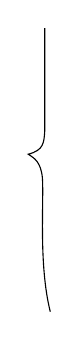
\begin{tikzpicture}\draw (.2,0)..controls(.05,.6)and(.12,1.4)..(.1,1.7)..controls(.08,1.9)and(0,1.95)..(-.08,2)..controls(.12,2.05)and(.12,2.15)..(.13,2.3)--(.13,3.6);\end{tikzpicture}}

\uline{Prop B} Localement au voisinage de chaque pt de $Y_i$, on a $(X,Y_i)\simeq Y_i\times(N_{\unsure{i|\xi}},a)$, où $\unsure{a|N}$ est un espace topologique dont $a$ est une singularité \uline{immobile}. [Le type d'homéomorphie locale de $(N,a)$ ne dépend que de la composante connexe du point envisagé de $Y_i$]
\margin{Vrai $\forall X$ \unsure{dévissable}, et alors \deleted{\unsure{alors}} $N$ est \unsure{dévissable}?}
\figure{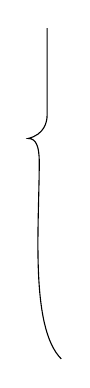
\begin{tikzpicture}\draw (.3,0)..controls(-.1,.4)and(.02,1.7)..(.02,2.5)..controls(.02,2.7)and(-.02,2.8)..(-.12,2.8)..controls(.08,2.85)and(.12,3)..(.12,3.1)--(.12,4.2);\end{tikzpicture}}

\uline{Prop C} Pour tt $x\in Y_i$, $(Y_i,\unsure{y|x})$ est le \deleted{\unsure{p}} plus gros germe de sous-variété \inserted{$Y$} de $X$ en $x$ le long de laquelle $X$ soit équisingulier. Tous les ``autres'' $Y$ correspondent \inserted{$\overset{1-1}{\longleftrightarrow}$} aux germes \inserted{en $x$ de} sous-variétés régulièrement immergées de $Y_i$. \deleted{\illegible{1}}
\mspage{28}
